% Use only LaTeX2e, calling the article.cls class and 12-point type.

\documentclass[12pt]{article}
% Users of the {thebibliography} environment or BibTeX should use the
% scicite.sty package, downloadable from *Science* at
% www.sciencemag.org/about/authors/prep/TeX_help/ .
% This package should properly format in-text
% reference calls and reference-list numbers.
\usepackage{geometry}
\usepackage{listings}
\usepackage{url,enumerate, amssymb, anysize, booktabs, amsfonts}
\usepackage[colorlinks = true,
linkcolor = blue,
urlcolor  = blue,
citecolor = green,
anchorcolor = blue]{hyperref}
\usepackage{setspace,listings}
%\usepackage{cite}
\usepackage[square,numbers]{natbib}
\bibliographystyle{abbrvnat, lipsum}
\usepackage{mathrsfs}
%\usepackage{hanging}
\renewcommand*\thesection{\arabic{section}}
\usepackage{color,amssymb}
\usepackage{fancyhdr, mathtools}
\usepackage{dcolumn}
\usepackage{indentfirst, verbatim}
\newcounter{equationset, sectsty, breqn}
\usepackage{setspace,float,lscape,amsmath,color}
\usepackage{outlines}
\usepackage[font=sf, labelfont={sf,bf}, margin=1cm]{caption}
\usepackage{amsthm}
\captionsetup{font={small,sf,singlespacing}}
\newcommand{\pb}{\mathbb{P}}
\newcommand{\E}{\ensuremath{\mbox{E}}}

\theoremstyle{definition}
\newtheorem{definition}{Definition}[section]
\newtheorem{theorem}{Theorem}[section]
\newtheorem{corollary}{Corollary}[theorem]
\newtheorem{lemma}[theorem]{Lemma}
\newtheorem{remark}{Remark}


% Page style definition
\geometry{margin=1.0in}
\pagestyle{fancy}
%\usepackage{scicite}

% Use times if you have the font installed; otherwise, comment out the
% following line.

\usepackage{times}

% The preamble here sets up a lot of new/revised commands and
% environments.  It's annoying, but please do *not* try to strip these
% out into a separate .sty file (which could lead to the loss of some
% information when we convert the file to other formats).  Instead, keep
% them in the preamble of your main LaTeX source file.



% The following parameters seem to provide a reasonable page setup.

\topmargin 0.0cm
\oddsidemargin 0.2cm
\textwidth 16cm 
\textheight 21cm
\footskip 1.0cm


%The next command sets up an environment for the abstract to your paper.

\newenvironment{sciabstract}{%
\begin{quote} \bf}
{\end{quote}}


% If your reference list includes text notes as well as references,
% include the following line; otherwise, comment it out.

\renewcommand\refname{References and Notes}

% The following lines set up an environment for the last note in the
% reference list, which commonly includes acknowledgments of funding,
% help, etc.  It's intended for users of BibTeX or the {thebibliography}
% environment.  Users who are hand-coding their references at the end
% using a list environment such as {enumerate} can simply add another
% item at the end, and it will be numbered automatically.

\newcounter{lastnote}
\newenvironment{scilastnote}{%
\setcounter{lastnote}{\value{enumiv}}%
\addtocounter{lastnote}{+1}%
\begin{list}%
{\arabic{lastnote}.}
{\setlength{\leftmargin}{.22in}}
{\setlength{\labelsep}{.5em}}}
{\end{list}}


% Include your paper's title here

\title{Testing independence between networks and nodal attributes via multiscale metrics and multiscale distance correlation} 

% Place the author information here.  Please hand-code the contact
% information and notecalls; do *not* use \footnote commands.  Let the
% author contact information appear immediately below the author names
% as shown.  We would also prefer that you don't change the type-size
% settings shown here.

\author
{John Smith,$^{1\ast}$ Jane Doe,$^{1}$ Joe Scientist$^{2}$\\
\\
\normalsize{$^{1}$Department of Chemistry, University of Wherever,}\\
\normalsize{An Unknown Address, Wherever, ST 00000, USA}\\
\normalsize{$^{2}$Another Unknown Address, Palookaville, ST 99999, USA}\\
\\
\normalsize{$^\ast$To whom correspondence should be addressed; E-mail:  ylee160@jhu.edu.}
}

% Include the date command, but leave its argument blank.

\date{}

%%%%%%%%%%%%%%%%% END OF PREAMBLE %%%%%%%%%%%%%%%%

\begin{document} 

% Double-space the manuscript.

\baselineskip24pt
\sloppy
% Make the title.

\maketitle 

% Place your abstract within the special {sciabstract} environment.

\begin{sciabstract}
 Network dependence over network space, which refers to the dependence between network topology and its nodal attributes, often exhibits nonlinear dependent properties. Unfortunately, without knowledge on specific neighborhood structures, no statistic has been suggested to test network dependence further than globally linear dependence. This paper introduces a multiscale dependence test statistic called Multiscale Network Test (\texttt{MNT}), which borrows the idea of diffusion maps and Multiscale Generalized Correlation (\texttt{MGC}). Our methodology for testing network independence to any multivariate nodal attributes can be applied to any exchangeable graph. We prove the consistency of \texttt{MGC} in this application and demonstrate better performance than any other model-based, global test statistics. 
\end{sciabstract}

\newpage

\textbf{Outlines}
\bigskip
\begin{outline}[enumerate]
\1 Abstract : 
\begin{itemize}
	\item This paper introduces the novel statistical methods to test independence between network and nodal attributes.

	\item KEY WORDS : multivariate independence test, diffusion maps, distance correlation, k-nearest neighbors,

\end{itemize}

\1 INTRODUCTION

\2 introduce interests in association between network and nodal attributes and the related literatures.
\begin{itemize}
\item explicitly state the problem and its importance, previous approaches' weakness. 
\item difference to previous/common approach, what is our specialty.
\end{itemize}

\2 Introduce notations we are going to use and introduce a common network model of nodal attributes.
\begin{itemize}
\item briefly explains the difficulties (how to represent network topology) and how we overcome them
\item introduce outlines
\end{itemize}

\1 METHODOLOGY

	\2 introduce a exchangeable graph
		\3 definition of exchangeable graph and lemmas under directed graph
		\3 explain difficulties in undirected or more general graph and introduce representation theorem
		\3 explains more general version of graph, i.e. graphex
		\3 state corollary that commonly used graphical models which satisfy exchangeability, e.g. SBM, RDPG, Fosdick's latent model

	\2 represent a network structures as a one-parameter family or multivariate variables
		\3 introduce notations and definition (coifman $\&$ ming)
		\3 explains spectral properties of diffusion maps
		\3 Lemmas about properties of diffusion maps under exchangeable graphs

	\2 introduce Dcor and MGC to apply testing independence G and X
		\3 introduce distance correlation and multiscale version
		\3 discuss the choice of proper metrics for testing network independence and demonstrate diffuion distance is appropriate.
		\3 present the main theorem and a few remarks.


\1 SIMULATION PERFORMANCE AND PRACTICAL IMPLEMENTATION

	\2 stochastic block model
		\3 simplest two block model
		\3 simplest three block model
		\3 sparse version of block model

	\2 random-dot product grap
		\3 simplest RDPG + "remarks" about consistent estimation on latent variable
		\3 comparison to Fosdick's method.	


\1 APPLICATION

(black box)


\1 CONCLUDING REMARKS

	\2 discuss merits of using MNT 
	\2 discuss limitations of using MNT
	\2 discuss possible contributions of MNT and future works



\1 APPENDIX


\1 REFERENCES


\1 SUPPLEMANTARY FIGURES

\end{outline}


% In setting up this template for *Science* papers, we've used both
% the \section* command and the \paragraph* command for topical
% divisions.  Which you use will of course depend on the type of paper
% you're writing.  Review Articles tend to have displayed headings, for
% which \section* is more appropriate; Research Articles, when they have
% formal topical divisions at all, tend to signal them with bold text
% that runs into the paragraph, for which \paragraph* is the right
% choice.  Either way, use the asterisk (*) modifier, as shown, to
% suppress numbering.
\newpage
\tableofcontents


%%%%%%%%%%%%%%%%%%%%%%%%%%%%%%%%%%%%%%%%%%%%%%%%%%%%%%%%%%%%%%%
\newpage

\section{Introduction}

\subsection{intro1}

Network, a collection of nodes and edges between them, has been a celebrated area of study over a field of psychology, information theory, biology, statistics, economics, etc. The relationship between the way a pair of nodes are connected and the values of their attribute is a common interest in network analysis. There has been a lot of efforts to represent a network as a function of nodal attributes or model an outcome of nodal attribute variables through their underlying network structures. However, it is very obscure to determine which one should be put as a dependent variable. And most of all network often does not have a natural structure. This is why there exist a plethora of works on latent structure of network, which also depends on the characteristics of each node ( \hyperlink{Hoff}{Hoff et al. (2002)}  , \hyperlink{Austin}{Austin, Linkletter, and Wu (2013)} ). In a latent space model, local independence between network and nodal attributes, conditional on a latent variable is often assumed ( \hyperlink{Lazarsfeld}{Lazarsfeld and Henry (1968)} ), which makes easier to interpret the dependency mechanism. In real network data, however, it is almost impossible to estimate such latent variable without any knowledge on true network generative model and also we cannot guarantee that direction or amount of association between network and nodal attributes keeps consistent across latent variables, i.e. we cannot guarantee linear dependence. 


\subsection{intro2}
 
 Throughout this paper, assume that we are given an unweighted and undirected, connected network $\boldsymbol{G}$ comprised of $n$ nodes, for a fixed $n \in \mathbb{N}$. Suppose that our observation of $\boldsymbol{G}$ is one random sample from true, population distribution of $\mathcal{G}$. Even though we assume that $\boldsymbol{G}$ is an undirected and unweighted network but we are able to extend all of the theory here to directed and even weighted network. An adjacency matrix of a given network, denoted by $\boldsymbol{A} = \{A_{ij} : i,j= 1,..,n \}$, is often introduced to formalize this relational data of network. Let us introduce a $m$-variate ($m \in \mathbb{N}$) variable for nodal attributes $\boldsymbol{X}  \in \mathbb{R}^{m}$ which we are interested in. Investigating correlation between $\boldsymbol{G}$ and $\boldsymbol{X}$ and testing whether their distributions are independent or not is the key focus in our study. 
 Even though distribution of graph $\boldsymbol{G}$ is often formalized through modeling adjacent relations $\{a_{ij} : i,j = 1,... , n \}$, we cannot directly use $\mathbf{A}$ in testing independence to $\mathbf{X}$, mostly due to difficulty of extracting vertex-wise topological information. Rather than regressing $a_{ij}$ on observed attribute values $x_{i}$ or $x_{j}$, [Fosdick and Hoff] proposed a latent variable model to estimate node-specific network factor which provides a one-to-one correspondence between $\boldsymbol{G}$ and $\boldsymbol{X}$ as well as reduces a dimension of network data. In their paper, Fosdick and Hoff also used these factors to test independence between $\boldsymbol{G}$ and $\boldsymbol{X}$ through testing independence between network factors and nodal attributes. However, the performance of this test would not be good enough when the relational data $\boldsymbol{A}$ does not have linear relationship to network factors or has a latent mixture model. Since we never know the structure of networks and the way they are related to other variables, there always exist a limitation on testing based on modeling network.
 
 In this paper without modeling nor estimating networks, we develop multiscale test statistics which are robust to both nonlinearity and high dimensionality. Multiscale is not avoidable because we view relationship or distance over network as dynamic process so we choose the optimal scale where distance in network space and distance in terms of attributes become most correlated each other. Thus basically we define a coordinate over network at each time in process and test independence to attributes $\mathbf{X}$. In the next methodology section \ref{sec:method}, we are going to define such multiscale distance and its properties, and test statistic using multiscale distance metrics will be followed. In section \ref{sec:sim}, we demonstrate best performance of our method compared to the existing under various circumstances through numerical results. Real data example in section \ref{sec:real} show one of the applications among many.  
 
 
  
%%%%%%%%%%%%%%%%%%%%%%%%%%%%%%%%%%%%%%%%%%%%%%%%%%%%%%%%%%%%%%%%
\newpage
\section{Methodology}
\label{sec:method}

First step in testing network independence to other variables is to figure out the variable which configurates location of vertices over network space.  We hope that our observed network be a realization of such variable so that our test results can be generalized to those from population of given network. Moveover a pair of our observations for each variable we are going to test should be i.i.d realization to guarantee representativeness and avoid redundant intra-dependence.  

\subsection{Exchangeable Graph}

\subsubsection{[EG1]}


Assuming that we are given one network, equivalently one graph, it is not clear to consider given network as an independent and identically distributed sample of some variable. It is true that if you consider each edge is i.i.d., then observed adjacency matrix is a random sample of  a single parameter which is the probability of having edge or not. However, in this case, the resulting network model only depends on number of edges \cite{Orbanz} and does not cover undirected or no self-loop networks.  

 The property of exchangeability is closely related to the use of independent and identically-distributed(i.i.d) random variable. Network or graph $\mathbf{G}$ is called exchangeable if and only if its adjacency matrix $\mathbf{A}$ is jointly exchangeable \cite{Orbanz}. 

\begin{definition}[2-array exchangeability]
	\label{exchangeability}
	A random 2-array $(A_{ij})$ is called $\mathbf{\mbox{jointly exchangeable}}$ if 
	$$(A_{ij}) \stackrel{d}{=} (A_{\sigma(i) \sigma(j)})$$
	for every permutation $\sigma$ of $n$,
	and separately exchangeable if 
	$$(A_{ij}) \stackrel{d}{=} (A_{\sigma(i) \sigma^{\prime}(j) })$$
	for every pair of permutation $\sigma, \sigma^{\prime}$ of $n$.
\end{definition}



\subsubsection{[EG2]}

However, exchangeability itself cannot guarantee being $i.i.d$. Fortunately, thanks to the celebrated  \textit{de Finetti}(\ref{finetti})'s representation theorem, it has been proven that there exists a random probability measure $\eta$ on random variable $\mathbf{Z}$ that a sequence of $Z_{1}, Z_{2}, ... $ are \textit{i.i.d} conditional $\eta$ \textit{if and only if} the sequence is exchangeable \cite{Orbanz} \cite{Caron}. \textit{Aldous-Hoover theorem}(\ref{Aldous_Hoover}) is the representation theorem of 2-array exchangeable array, which would be useful to explain jointly exchangeable adjacent matrix. Exchangeable graph is commonly called \textit{graphon}. Exchangeable graphon is defined through a random measurable functions follows \cite{Chan}:

\begin{definition}[graphon]
	\label{graphon}
	
	A \textit{graphon} with $n (\in \mathbb{N})$ nodes is defined as a function of a symmetric measurable function $g : [0,1]^2 \rightarrow [0,1]$ with input of $u_{i} \overset{i.i.d}{\sim} Uniform[0,1], i = 1,2,... ,n$. 
	Let $\mathbf{A}$ be an adjacency matrix of graphon. Then for any $i \leq j, i,j=1,2,...,n$:	
	\begin{equation}
	Pr \big(   A_{ij} = 1 \big| u_{i}, u_{j} \big) = g \big(  u_{i}, u_{j} \big)
	\end{equation}
	
\end{definition}

Thanks to \textit{Aldous-Hoover theorem}, we can now better represent exchangeable network through measurable function, but we are still halfway done in case of undirected network where $A_{ij} = A_{ji}$  $(i,j=1,2,... , n)$.  Under undirected network where self-loop is still allowed, we can represent $\{ A_{ij} : i \leq j \}$ as a function of $g$ conditioning on $\{ u_{i}\}$. 
In the next section, we will explain the shortcomings of representing network as a graphon and introduce more general exchangeable graph in the next. 

\begin{equation}
( A_{ij} )  =  (   A_{\sigma(i) \sigma(j)}  ) \Longleftrightarrow A_{ij} \overset{ind}{\sim} Bern\big(  g(u_{i}, u_{j}) \big), i \leq j
\end{equation}  


\subsubsection{[EG3]}

Graphon has been studied widely as a limit of random graphs \textcolor{red}{(ref : )}. However, despite its advantage on simple representation, is either empty or dense. Thus it fails to represent real network data where sparsity or scale-free distribution if fairly common. In addition to graphon,we introduce a concept of \textit{graphex}, first proposed by \href{http://arxiv.org/abs/1512.03099}{Veitch and Roy, 2015}\cite{Veitch}, which is more generalized version of graphon and also includes sparse exchangeable graphs \cite{Caron}. A trick \hyperlink{Caron}{Caron and Fox} used is representing a network as a point process on $\mathbb{R}^2_{+}$ based on \textit{Kallengerg Representation Theorem}\cite{Kallenberg}. Like we are able to represent $\{ A_{ij} \}$ through random transformation of \textit{i.i.d} uniform variables, jointly exchangeable point processing network also can be represented via a random function of \textit{i.i.d} unit rate Poisson process and uniform variables. 
	To be specific, undirected graph on a point process on $\mathbb{R}^2_{+}$ can be thought of 
\begin{equation}
\mathbf{A} = \sum\limits_{i,j} A_{ij} \delta_{( \theta_{i}, \theta_{j})} 
\end{equation}	
,where $A_{ij} = A_{ji} \in \{ 0 , 1  \}$ with $\theta_{i} \in \mathbb{R}$, $i,j = 1,2,...$. We can think \texttt{Node} $i$ is embedded on real line, at $\theta_{i} \in \mathbb{R}_{+}$. 	


\begin{definition}[Joint exchangeability on point process]
	\label{point}
Let $h > 0$ and  $V_{i} = [h(i-1), hi ]$ for $i \in \mathbb{N}$ then
\begin{equation}
\big( A( V_{i} \times V_{j}  )   \big)  \stackrel{d}{=} \big( A( V_{\sigma(i)} \times V_{\sigma(j)}     \big)
\end{equation}	
for any permutation $\sigma$ of $\mathbb{N}$.		
\end{definition}








\begin{definition}[graphex (Veitch and Roy, 2015)]
	\label{graphex}
	
	

	
\end{definition}







\subsubsection{[EG4]}


Widely used graphical model, e.g. Stochastic Block Model (SBM), Random Dot Product Graph (RDPG), satisfies this definition of jointly exchangeable graph under some constraints. 



\subsection{Multiscale Distance Metrics}


\subsubsection{[MDM1]}


There have been a lot of efforts to represent the network in terms of a summarizing network factor\cite{Hoff} or some meaningful coefficients, e.g. centrality\cite{centrality1}\cite{centrality2}. However, there has been no vertex-wise variable which provides a configuration of vertex over network space without losing any information. \hyperlink{Coifman}{Coifman $\&$ Lafon}\cite{Coifman} demonstrated that diffusion maps provide a meaningful multiscale geometries of data while keeping information on every local relation. Diffusion map is constructed via Markov chain on graph. Here an adjacency matrix $\boldsymbol{A}$ acts as a kernel, representing a similarity between each node in $\boldsymbol{G}$; thus we do not have to estimate anything to obtain multidimensional representation of network topology through diffusion maps. 

Let $(\boldsymbol{G}, \mathcal{A}, \mu)$ be a measure space. Throughout all of the arguments, assume that we have a countable vertex set with size of $n \in \mathbb{N}$. The vertex set of network $\boldsymbol{G}$ is the data set of vertices and edges and $\mathcal{A}$ is a set of a pair of nodes $\{(i,j) : v_{i}, v_{i} \in V(\boldsymbol{G}) \}$. A measure of $\mu$ which represents a distribution of the vertices on $\boldsymbol{G}$, is equivalent to an adjacency matrix $\boldsymbol{A}$. A transition matrix $\mathbf{P} = \{P[i,j] : i,j=1,...,n \}$ in Markov chain on $\boldsymbol{G}$, which represents the probability that flow or signal goes from Node $i$ to Node $j$, is defined as below:

\begin{equation}
P[i,j] = A_{ij} \big/ \sum\limits_{j=1} A_{ij}
\end{equation}

A transition matrix $\mathbf{P}$ is a new kernel of a Markov chain of which element $P[i,j]$ represents the probability of travel from Node $i$ to Node $j$ in one time step. On the other hand, corresponding probability in $t$ steps is given by the $t$ th ($t \in \mathbb{N}$) power of $P$. How to derive diffusion distance over a directed network or weighted network is provided in [Tang $\&$ Trosset (2010)]. Other than a transition matrix, we need a stationary probability $\boldsymbol{\pi} = \{\pi(1), \pi(2), ... , \pi(n) \}$ of which $\pi(i)$ represents the probability that the chain stays in Node $i$ regardless of the starting state. In our setting, $\pi(i)$ is proportional to the degree of Node $i$, i.e. $\pi(i) = \sum\limits_{j=1}^{n} A_{ij} \big/ \sum\limits_{i=1}^{n}\sum\limits_{j=1}^{n} A_{ij}$ ($i=1,2,..., n$).   

For each time point $t \in \mathbb{N}$, we can define a diffusion distance $C_{t}$  given by :

\begin{equation}
\begin{split}
C^2_{t}[i,j] & = \sum\limits_{w =1}^{n} \big( P^{t}[i,w] - P^{t}[j,w]  \big)^{2} \frac{1}{\pi(w)} = \sum\limits_{w=1}^{n} \left(  \frac{P^{t}[i,w]}{\sqrt{\pi(w)}} - \frac{P^{t}[j,w]}{\sqrt{\pi(w)}}   \right)^2 \\ & = \parallel P^{t}[i, \cdot] - P^{t}[j, \cdot]  \parallel^2_{L^{2}(\boldsymbol{G}, d\mu / \pi)  }
\end{split}
\end{equation}

As diffusion time $t$ increases, distance matrix $C_{t}$ is more likely to take into account distance between two nodes far away in terms of the length of the path. Key idea behind such diffusion distance at fixed time $t$ is that it measures the chance that we are likely to stay between \texttt{Node i} and \texttt{Node j} at $t$ step on our journey of all other possible paths. The higher chance is, the smaller distance between two is. This distance well reflects the connectivity between two nodes. Connectivity between two nodes is higher if we need to eliminate more number of vertices to disconnect these two. Unlike an adjacency relation or geodesic distance, a connectivity between two nodes depends on their relationship to other vertices in a given network so it is more robust to the unexpected edges. Often a set of nodes with higher connectivity have a higher propensity of having edges within this set and they are likely to form a cluster. Thus diffusion distance is very robust measure and also very sensitive to the clustering structure of network. 



\subsubsection{[MDM2]}

Diffusion distance of $\boldsymbol{G}$ defined as above can be represented via a spectral decomposition of its transition matrix $P$. That is, we can derive diffusion distance using its eigenvectors and eigenvalues. The spectral analysis on diffusion distance or diffusion maps have been studied for its usefulness for nonlinear dimensionality reduction ([Coifman $\&$ Lafon (2006)], [Lafon $\&$ Lee (2006)]). 
Keeping mind that diffusion distance at time $t$, $C_{t}$ is a functional $L^2$ distance, weighted by 1/$\pi$. If we transform the way to represent $C_{t}[i,j]$ slightly, we are able to obtain an orthonormal basis of $L^{2}(\mathbf{G}, d\mu / \pi)$ via eigenvalues and eigenvectors. 
Since an adjacency matrix $A$ does not guarantee a symmetric of $P$, define a symmetric kernel $\boldsymbol{Q} = \boldsymbol{\Pi^{1/2} P \Pi^{-1/2}},$ where $\mathbf{\Pi}$ is a $n \times n$ diagonal matrix of which $i$th diagonal element is $\pi(i)$. Under compactness of $P$, $\boldsymbol{Q}$ has a discrete set of real nonzero eigenvalues $\{ \lambda_{r} \}_{r = \{1,2,...,q \}}$ and a set of their corresponding orthonormal eigenvectors $\{ \psi_{r} \}_{r = \{1,2,..., q \} },$ i.e. $Q[i,j] = \sum\limits_{r=1}^{q} \lambda_{r} \psi_{r}(i) \psi_{r}(j)$ ($1 \leq q \leq n$).  
 Since $P[i,j] = \sqrt{\pi(j) / \pi(i) } Q[i,j]$, $P[i,j]= \sum\limits_{r=1}^{q} \lambda_{r} \{ \psi_{r}(i) / \sqrt{\pi(i)}  \} \{ \psi_{r}(j) \sqrt{\pi(j)} \} := \sum\limits_{r=1}^{q} \lambda_{r} \phi_{r}(i) \{ \psi_{r}(j) \sqrt{\pi(j)} \}$, where $\phi_{r}(i) := \psi_{r}(i) / \sqrt{\pi(i)}$. Then from $\sum\limits_{r=1}^{q} \psi_{r}(j) \sqrt{\pi(j)} = 1$ for all $j \in \{1,2,...,n\}$, 
 we can represent the diffusion distance as: 
 
 \begin{equation}
 \begin{split}
 C^2_{t}[i,j] & = \sum\limits_{r=1}^{n} \lambda^{2t}_{r} \big( \phi_{r} (i) - \phi_{r}(j)   \big)^2   \\ &  = \parallel P^{t}[i, \cdot] - P^{t}[j, \cdot]  \parallel^2_{L^{2}(\boldsymbol{G}, d\mu / \pi)  }
 \end{split}
 \end{equation}
 
 That is,
 
 \begin{equation}
 C_{t}[i,j] = \parallel \boldsymbol{U}_{t}(i) - \boldsymbol{U}_{t}(j) \parallel
 \end{equation}
 , where 

\begin{equation} 
 \boldsymbol{U}_{t}(i) = \begin{pmatrix} \lambda^{t}_{1} \phi_{1}(i) \\ \lambda^{t}_{2} \phi_{2} (i)  \\ \vdots \\ \lambda^{t}_{q} \phi_{q}(i) \end{pmatrix} \in \mathbb{R}^{q}.
 \end{equation}


Now we call the family of $q$-variate($q \leq n$) diffusion maps $\{ U_{t} \}_{t \in \mathbb{N}} $, of which Euclidean distance is diffusion distance.


\subsubsection{[MDM3]}
\begin{itemize}
	\item {\it  [MDM3] properties of diffusion maps under exchangeable graphs \/}
\end{itemize}

Due to the inter-correlated construction of $U$, e.g. $i$th subject's diffusion depends on others in the given network, it is hard to say that the observed diffusion coordinates of $n$ subjects are independent samples without any restrictions on networks. Independence within sample of one variable is important in testing independence with other variable. (\textcolor{red}{why? example})

To talk about independence of $U$, we need more general concept of exchangeable graph. Remind that under jointly exchangeable graph, $(A_{ij}) \stackrel{d}{=} (A_{\sigma(i) \sigma(j)})$
for every permutation $\sigma$ of $n$. The main advantage from such representation of $\mathbf{A}$ is that it becomes now possible to represent given network $\boldsymbol{G}$ as a one-parameter family of $q(<n)$-coordinates called diffusion coordinate, of which metric well reflects how corresponding vertices are connected each other at each diffusion time point. A set of diffusion maps for each vertex have some desirable properties which will be helpful in testing. The followings are concerning about a few conditions for earning them. 

\begin{lemma}[Exchangeability and i.i.d. of $A$ in graphon]
	\label{lemma1}
	Assume that a connected, undirected and unweighted graph $\mathbf{G}$ is a graphon. Then 2-array of $\{ A_{ij} : i = 1,2,... ,n , i \leq j \}$ are i.i.d. conditioning on random link function $g : [0,1]^2 \rightarrow [0,1]$. Thus for fixed row (column) of $\mathbf{A}$, $\{ A_{i1}, A_{i2}, ... , A_{in} \}$, $i \in \{ 1,2,... , n \}$ are conditionally i.i.d. on random link function $g$.  
\end{lemma}



\begin{lemma}[Exchangeability and i.i.d. of $A$ in graphex]
	\label{lemma2}
	Assume that a connected, undirected and unweighted graph $\mathbf{G}$ is a graphex. Then 2-array of $\{ A_{ij} : i = 1,2,... ,n , i \leq j \}$ \textcolor{red}{need cautions}
\end{lemma}


From the above Lemma \ref{lemma1}, \ref{lemma2}, we can also prove exchangeability and conditional i.i.d. of diffusion maps at each time point. 

\begin{lemma}[Exchangeability and iid of $U$]
	\label{lemma3}
Assume that a connected, undirected and unweighted graph $\mathbf{G}$ is a graphon or graphex, i.e. any exchangeable random graph from an infinite graph. Then its transition probability $P_{ij}$ so thus  diffusion maps at fixed time $t$ also exchangeable conditional on link function of graph. Furthermore, by [de Finetti]'s Theorem\ref{finetti}, we can say that such diffusion maps at $t$ are conditionally i.i.d given random probability measure $\eta$ on $U_{t}$ and random link function $g$.    
\end{lemma}


Lemma \ref{lemma3} above provides us i.i.d. one-parameter family of $\{ \mathbf{U}_{t} \}_{t \in \mathbb{N}}$ conditional on a random probability measure of $\mathbf{U}_{t}$ and a random link function of $g$.


%%%%%%%%%%%%%%%%%%%%%%%%%%%%%%%%%%%%%%%%%%%%%%%%%%%%%%%%%%%%%%%%
\newpage
\subsection{Multiscale Generalized Correlation}

\subsubsection{[MGC1]}


Relationship between network and nodal attributes often exhibits local or nonlinear properties. Moreover, dimension of spectrum of network$(q)$ increases as a sample size increases. Unfortunately, widely used correlation measures often fail to capture nonlinear associations or multivariate associations. Szekely et al. (2007)\cite{Szekely2007} extended pairwise constructed generalized correlation coefficient and developed a novel statistics called distance correlation (\texttt{dCov}) as a measure for all types of dependence between two random vectors in any dimension. Let us first start from a general setting that we are given $n \in \mathbb{N}$ pairs of random samples $\{ (x_{i}, y_{i}) : x_{i} \in \mathbb{R}^{q}, y_{i} \in \mathbb{R}^{m}, i = 1,...,n \}$. Define $C_{ij} = \parallel x_{i} - x_{j} \parallel$ and $D_{ij} = \parallel y_{i} - y_{j} \parallel$ for $i,j=1,...,n$, where $\parallel \cdot \parallel$ denotes Euclidean distance defined on any vectors.   
Distance correlation (\texttt{dCor}) is defined via distance covariance (\texttt{dCov}) $\mathcal{V}^2_{n}$ of $\boldsymbol{X}$ and $\boldsymbol{Y}$, which is the following: 

\begin{equation}	 
\mathcal{V}^2_{n}(\boldsymbol{X}, \boldsymbol{Y}) = \frac{1}{n^2} \sum\limits_{i,j=1}^{n} \tilde{C}_{ij} \tilde{D}_{ij}
\end{equation}
, where $\tilde{C}$ and $\tilde{D}$ is a doubly-centered $C$ and $D$ respectively, by its column mean and row mean. Distance correlation $\mathcal{R}^{2}_{n}(\boldsymbol{X}, \boldsymbol{Y})$ is a standardized \texttt{dCov} by $\mathcal{V}^2_{n}(\boldsymbol{X}, \boldsymbol{X})$ and $\mathcal{V}^2_{n}(\boldsymbol{Y}, \boldsymbol{Y}).$

\begin{equation}	 
\mathcal{R}_{n}^{2} (\boldsymbol{X}, \boldsymbol{Y}) = \frac{\mathcal{V}^2_{n} (\boldsymbol{X}, \boldsymbol{Y}) }{\sqrt{\mathcal{V}^2_{n} (\boldsymbol{X}, \boldsymbol{X}) \mathcal{V}^2_{n} (\boldsymbol{Y}, \boldsymbol{Y}) } }
\end{equation}
	 
On the other hand, a modified distance covariance (\texttt{MCov}) $\mathcal{V}^*_{n}$ and a modified distance correlation (\texttt{MCorr}) $\mathcal{R}^{*}_{n}$ for testing high dimensional random vectors were also proposed in Szekely et al. (2013)\cite{Szekely2013}.   
However, \texttt{dCov} and even \texttt{MCorr} still perform not very well in existence of various nonlinear dependency and under existence of outliers (\cite{Cencheng}). Out of this concern, Cencheng at al (2016) \cite{Cencheng} developed Multiscale Generalized Correlation (\texttt{MGC}) by adding local scale on correlation coefficients. Multiscale version of distance covariance $\{ { {\mathcal{V}^{*}}^2_{n} }   \}_{kl}$ is defined as following : 
	
\begin{equation}
\label{eq:MGC}
{\mathcal{V}^{*}}^2_{n} (\boldsymbol{X}, \boldsymbol{Y})_{kl} = \frac{1}{n^2} \sum\limits_{i,j=1}^{n} \tilde{C}_{ij} \tilde{D}_{ij} I \big( r(C_{ij}) \leq k \big) I \big( r(D_{ij})) \leq l  \big), \quad k,l=1,2,..., n 
\end{equation}
,where $r(C_{ij})$ ($r(D_{ij})$) is a rank $\mathbf{x}_{i}$ ($\mathbf{y}_{i}$) relative to $\mathbf{x}_{j}$ ($\mathbf{y}_{j}$). We basically truncate each pairwise element of distance covariance with respect to rank in terms of (Euclidean) distance. Note that if $k=l=n$, $\mathcal{V}^2_{n}$ and ${\mathcal{V}^{*}}^2_{n}$ are equivalent. Since we call all family of $\{  {\mathcal{R}^{*}}^2_{n} \}_{k,l = 1,2,...,n}$ as \texttt{MGC} and choose the optimal set of neighborhood choice of $(k,l)$, \texttt{MGC} is more generalized version of \texttt{dCor}. Its superiority and consistency have been proven against all alternatives \cite{Cencheng}. Particularly, in simulation\ref{sec:sim} we are going to show in which pattern of underlying dependency exists \texttt{MGC} is much more sensitive than global scale of statistics. 


\subsubsection{[MGC2]}


Returning to the problem of network setting, the fundamental problem is in measuring all types of dependence between $\boldsymbol{G}$ and $\boldsymbol{X}$ via \texttt{MGC}, we are required a \textit{i.i.d.} vertex-wise coordinates of which Euclidean distance measures a distance between them. You might first propose directly using a column of an adjacency matrix so that we have a $n$-pair of observations $\big\{ \big( \boldsymbol{A}_{i \cdot} , \boldsymbol{X}_{i} \big) : \boldsymbol{A}_{i \cdot} = (A_{i 1} , ... , A_{i n} ), \boldsymbol{X}_{i} \in \mathbb{R}^{m}, i=1,...,n  \big\}.$ In an undirected graph, $\{ \mathbf{A_{i \cdot}}  \}$ cannot be independent. Even if it is in e.g. directed graph, Euclidean distance between $\{ \boldsymbol{A}_{i \cdot} : i =1, ... , n \}$ is not a proper metric over network space. Let us introduce a simple example. Let a given network $\boldsymbol{G}$ having 8 nodes be an unweighted, directed network and possibly having self-loop. Let $\boldsymbol{A}$ be its $8 \times 8$ binary adjacency matrix. Assume \texttt{Node 1}, \texttt{Node 4} and \texttt{Node 8} have the following row entries:

\begin{equation}
\begin{gathered}
\boldsymbol{A}_{1 \cdot} = \left( \begin{array}{rrrrrrrr} 1 & 1 & 1 & 1 & 1 & 1 & 1 & 1 \end{array} \right) \\
\boldsymbol{A}_{4 \cdot} = \left( \begin{array}{rrrrrrrr} 1 & 1 & 1 & 1 & 0 & 0 & 0 & 0 \end{array} \right) \\
\boldsymbol{A}_{8 \cdot} = \left( \begin{array}{rrrrrrrr} 1 & 0 & 0 & 0 & 0 & 0 & 0 & 0 \end{array} \right)
\end{gathered}
\end{equation}

,which results $\parallel \boldsymbol{A}_{1 \cdot} -\boldsymbol{A}_{4 \cdot} \parallel^2 = 4$, $\parallel \boldsymbol{A}_{1 \cdot} -\boldsymbol{A}_{8 \cdot} \parallel^2 = 7$,and $\parallel \boldsymbol{A}_{4 \cdot} -\boldsymbol{A}_{8 \cdot} \parallel^2 = 3.$ Accordingly, $\parallel \boldsymbol{A}_{4 \cdot} -\boldsymbol{A}_{8 \cdot} \parallel  < \parallel \boldsymbol{A}_{1 \cdot} -\boldsymbol{A}_{4 \cdot} \parallel$. However, you can easily see that this does not make sense because \texttt{Node 4} and \texttt{Node 8} are connected each other only through \texttt{Node 1}. 
Therefore instead of using an adjacency matrix directly, we are considering embedding a vertex $v \in V(\boldsymbol{G})$ into its diffusion map of $\boldsymbol{U}$ and apply Euclidean distance metric, which is exactly a diffusion distance. As explained before, its Euclidean distance takes into account all possible paths between every pair of node and measure the connectivity between them. Unlike in the other metrics in network, i.e. adjacency matrix or geodesic distance, triangle inequality holds in diffusion distance (proof in [Appendix]). 

\begin{corollary}[Triangle inequality]
\label{corollary1}
For fixed time $t$, let $C_{t} : V(\mathbf{G})^2 \rightarrow \mathbb{R}_{+}$ be a diffusion distance defined on a pair of vertices in any connected and undirected graph $\mathbf{G}$. Then for any $v, w, z \in V(\mathbf{G})$,  
\begin{equation}
C_{t}(v,z) \leq C_{t}(v,w) + C_{t}(w,z)
\end{equation}
\end{corollary}	

Thanks to these properties of diffusion maps, we have better interpretation of its Euclidean distance so that we will use it to the distance matrix in \texttt{MGC}.

\subsubsection{[MGC3]}


We have discussed one-parameter family \textit{i.i.d.} representation of network structures, called diffusion maps, and also discussed when given \textit{i.i.d}. pair of observations of two variables, how distance correlation and its multiscale version test independence between these two. Now it is time to combine these two to test independence between network structures and nodal attributes efficiently and effectively.

\begin{theorem}[MGC of testing independence]
	\label{theorem1}
Assume that a connected, undirected and unweighted graph $\mathbf{G}$ is an exchangeable graph.  Assume that we are given $n$-pair of observations $\{ (u^{(t)}_{i}, x_{i}): i = 1,2,... , n  , t \in \mathbb{N} \}$. Then $u_{t}(i) \overset{i.i.d.}{\sim} f_{U_t} \big(  \eta, g \big)$, $t \in \mathbb{N}$ and $x_{i} \overset{i.i.d.}{\sim} f_{X}$, where $f_{U_t} \big( \eta, g \big)$ are conditional distribution function given a link function $g$ and a random probability measure $\eta_{t}$ of $U_t$. Then \texttt{MGC} applied to these pair of data is theoretically consistent against all dependent alternatives in testing :
$$H_{0} : f_{U_t \cdot X} = f_{U_t} \cdot f_{X}$$
\end{theorem}


Since $\boldsymbol{U}$ provides a configuration of vertices in $\boldsymbol{G},$ the above hypothesis implies testing independence between the configuration of vertices in network space and in attribute space, but as a function of a link function $g$ and a random function (variable) of $\eta$ of $\mathbf{U}$.


\begin{remark}
Roughly speaking, we can say that diffusion maps are i.i.d. function of a link function $g$ and a random function of $\mathbf{U}$, $\eta$. Thus testing independence between conditional $U$ and $X$ can be considered as testing independence between $f \big( g, \eta \big)$ and $X$. A link function $g$ concerns the distribution of edges and a random function $\eta$ concerns nature distribution of diffusion maps. Our testing basically examines whether how edges are constructed and how diffusions(propagation) process are correlated to nodal attributes.  
\end{remark}

%%%%%%%%%%%%%%%%%%%%%%%%%%%%%%%%%%%%%%%%%%%%%%%%%%%%%%%%%%%%%%%%
\newpage
\section{Simulation Study}
\label{sec:sim}

In simulation studies presented in this paper, we make a comparison of estimated testing power across various multivariate independence test statistics: \texttt{MGC}, \texttt{dCov}, Heller-Heller-Gorfine (\texttt{HHG})\cite{HHG}, and likelihood ratio test of Fosdick and Hoff (\texttt{FH}). For computing statistical power, we used type I error $\alpha = 0.05$ and obtain p-values of each sample network via permutations. For fair comparison between these testing methods, we also present a additive model of latent factors, which is mostly targeted by \texttt{FH}.   

\subsection{[sim1] Stochastic Block Model}
\begin{itemize}
	\item {\it  [sim1] present simplest examples of stochastic block model (graphon/graphex) \/}
\end{itemize}

 We mentioned in the Introduction that latent network model is very common followed by the assumption of local independence. Stochastic Block Model (SBM) is one of the most popular and also useful network generative model, especially as a tool for community detection ([Karrerl and Newman]). The SBM, in the simplest setting, assumes that each of $n$ vertices in graph $\boldsymbol{G}$ belongs to one of $K \in \mathbb{N} (\leq n)$ blocks or groups. Block affiliation is important because the probability of having edges between a pair of vertices depends on which blocks they are in. 
 
 Assume that the latent variable $Z_{1}, Z_{2}, ... , Z_{n} \overset{i.i.d.}{\sim} Multinomial\big( \pi_{1}, \pi_{2}, ... , \pi_{K} \big)$. Then the uppwer triangular entries of $\mathbf{A}$ are independent with 
 $A_{ij} \overset{i.i.d.}{\sim} Bern\big( \sum\limits_{k,l=1}^{K} p_{kl} I\big( Z_{i} = k, Z_{j} = l  \big)    \big), \forall  i < j$.
 
 Let $W_{1}, W_{2}, ... , W_{n} \overset{i.i.d.}{\sim} Unif[0,1]$. Then such $\mathbf{A}$ can be represented with respect to $\{ W_{i} \}$ as follows:

\begin{equation} 
A_{ij} \overset{i.i.d.}{\sim} Bern \big( g(W_{i}, W_{j})  \big), \forall i < j
\end{equation}
 , where $g\big( W_{i}, W_{j} \big) = \sum\limits_{k,l=1}^{K} p_{kl} I \big( W_{i} \in [\sum\limits_{j=1}^{k-1} \pi_{j}, \sum\limits_{j=1}^{k} \pi_{j}   ] , W_{j} \in [\sum\limits_{j=1}^{l-1} \pi_{j}, \sum\limits_{j=1}^{l} \pi_{j}  ]  \big)$


\subsubsection{[sim1.1] simplest two block model}

\begin{equation}
\begin{gathered}
X_{i} \overset{i.i.d}{\sim} Bern(0.5), i = 1,... , n \\ 
Z_{i}  \sim  \left\{  \begin{array}{cc} Bern(0.6) & X_{i} = 0 \\ Bern(0.4) & X_{i} = 1  \end{array} \right. \\
A_{z_{i}, z_{j}} \sim Bern \left[  \begin{array}{cc}   0.4 & 0.1  \\ 0.1 & 0.4 \end{array}  \right]
\end{gathered}
\end{equation}


\textcolor{red}{figure which compares power of MGC/dCov/hhg/FH}



\subsubsection{[sim1.2] simplest three block model}


\begin{equation}
\begin{gathered}
X_{i} \overset{i.i.d}{\sim} Multi(1/3, 1/3, 1/3), i = 1,2, ... , n \\ 
Z_{i}  \sim  \left\{  \begin{array}{ccc} Multi(1/2, 1/4, 1/4) & X_{i} = 1 \\ Multi(1/4, 1/2, 1/4) & X_{i} = 2 \\ Multi(1/4, 1/4, 1/2) & X_{i} = 3  \end{array} \right. \\
A_{z_{i}, z_{j}} \sim Bern \left[  \begin{array}{ccc}   0.5 & 0.2 &  0.3  \\ 0.2 & 0.5 & 0. 2  \\ 0.3 & 0.2 & 0.5  \end{array}  \right]
\end{gathered}
\end{equation}

\textcolor{red}{comparison to patter of power of MGC/dCov/hhg/FH from "simple" three block graph - figures in appendix}


\textcolor{red}{explain briefly why local optimal performs better in this case}


\textcolor{red}{figure which compares power of MGC/dCov/hhg/FH}



\subsection{[sim] other version of graph generation}


\subsubsection{[sim2.1] degree-corrected stochastic block model}

Under SBM, we assume that all nodes within the same block have the same expected degree. However, this block model is limited by homogeneous distribution within block and provides a poor fit to networks with hubs or highly varying node degrees within blocks or communities, which are common in practice. On the other hand, the Degree-Corrected Stochastic Block model (DCSBM) adds an additional set of parameter, often denoted by $\theta$, to control the node degrees. This model allows variation in node degrees within a block while preserving the overall block community structure. 








\textcolor{red}{figure which compares degree distribution of SBM vs. DCSBM}



\subsubsection{[sim2.2] exchangeable graph on Poisson process}


\textcolor{red}{simulation study explained in Veitch and Roy, 2015}
Sample a (latent) unit rate Poisson process $\Pi$ on $\theta \times \vartheta \in [0, \nu] \times [0, c]$.
 
\begin{equation}
\begin{gathered}
N_{\nu} \sim Poi( c \nu) \\ 
\{ \theta_{i} \} \big| N_{\nu} \overset{iid}{\sim} Uniform[0, \nu]  \\ 
\{ \vartheta_{i} \} \big| N_{\nu} \overset{iid}{\sim} Uniform[0,1] \\ 
\{ X_{i}  \} | N_{\nu} \overset{ind}{\sim} Normal \big( \vartheta_{i}, 0.1 \big)  \\ 
(\theta_{i}, \theta_{j}) \big| W, \vartheta_{i}, \vartheta_{j} \overset{ind}{\sim} Bernoulli \big( W\big( \vartheta_{i}, \vartheta_{j} \big) \big) 
\end{gathered}
\end{equation}





\subsubsection{[sim2.3] comparison to Fosdick's method}


Fosdick and Hoff proposed a approach of jointly modelling network and its attributes, where networks represent additional structure via sender-specific(or row-specific) and receiver-specific(or column-specific) latent factors.

As a connection to RDPG, this model can also represented as a product of combined latent factor $\tilde{u}$ and $\tilde{v}$. 

(factor additive model)

\begin{equation}
\begin{gathered}
u_{i} \overset{i.i.d}{\sim} Uniform[0,1] \\ 
A_{ij}  \overset{i.i.d}{\sim} Bern \big(  ( 1 - u_{i})^2 \times (1 - u_{j})^2    \big)
\end{gathered}
\end{equation}



Additionally some noise could be introduced as well due to artificially added edges to construct a connected graph.






%%%%%%%%%%%%%%%%%%%%%%%%%%%%%%%%%%%%%%%%%%%%%%%%%%%%%%%%%%%%%%%%
\newpage
\section{Real Data Examples}
\label{sec:real}

\subsection{MRI}

look into one largest connected component. 

$\{ \mathbf{U}_{t} \in \mathbb{R}^{q} \}_{t \in \mathbb{N}}$ $\mathbf{X} = (x,y,z) \in \mathbb{R}^{3}$

(it turns out that $q=$ )?

test what? test independence between brain network and its 3-dimensional locations; test independence between functional location and physical location. 

\begin{figure}[H]
	\label{fig:mri}
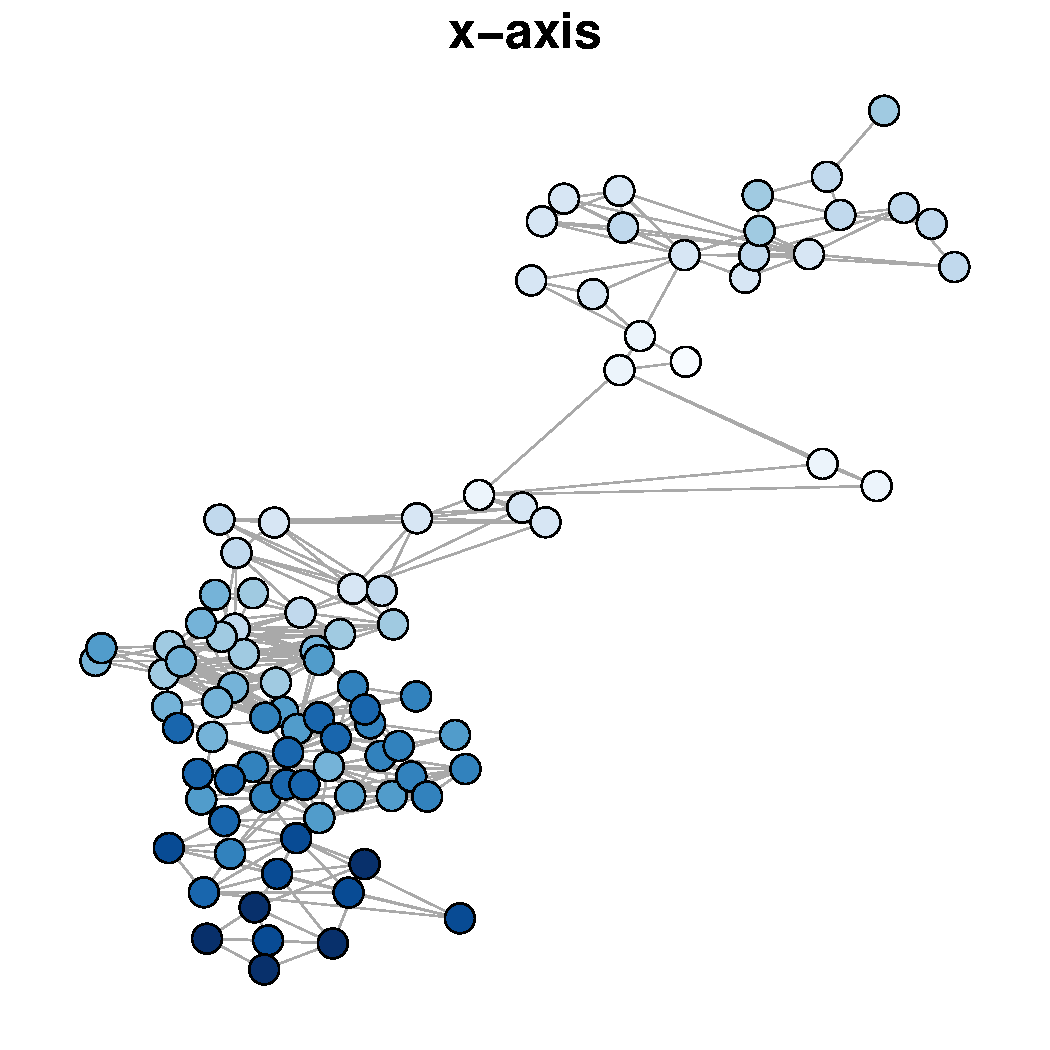
\includegraphics[width = 0.3\textwidth]{../Figure/brain1_x.pdf}
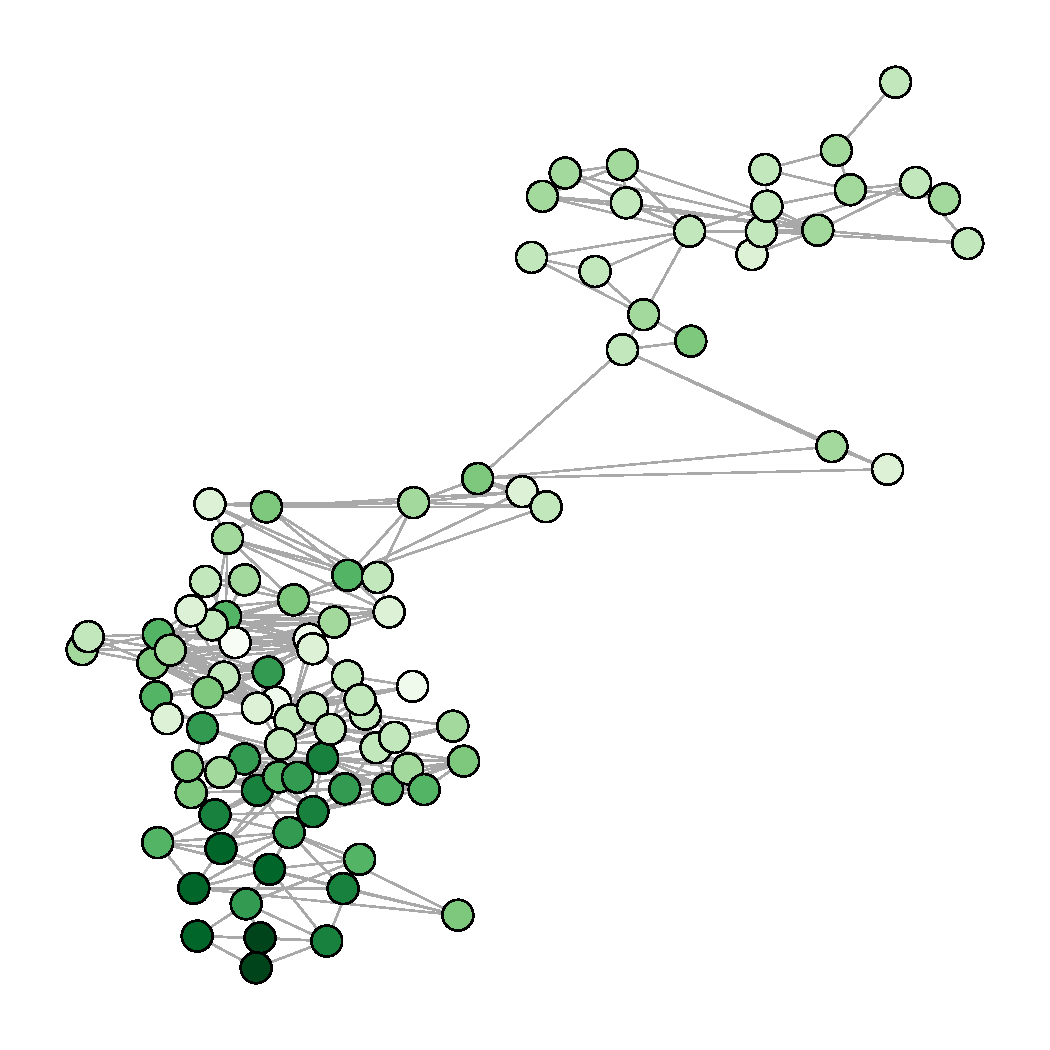
\includegraphics[width = 0.3\textwidth]{../Figure/brain1_y.pdf}
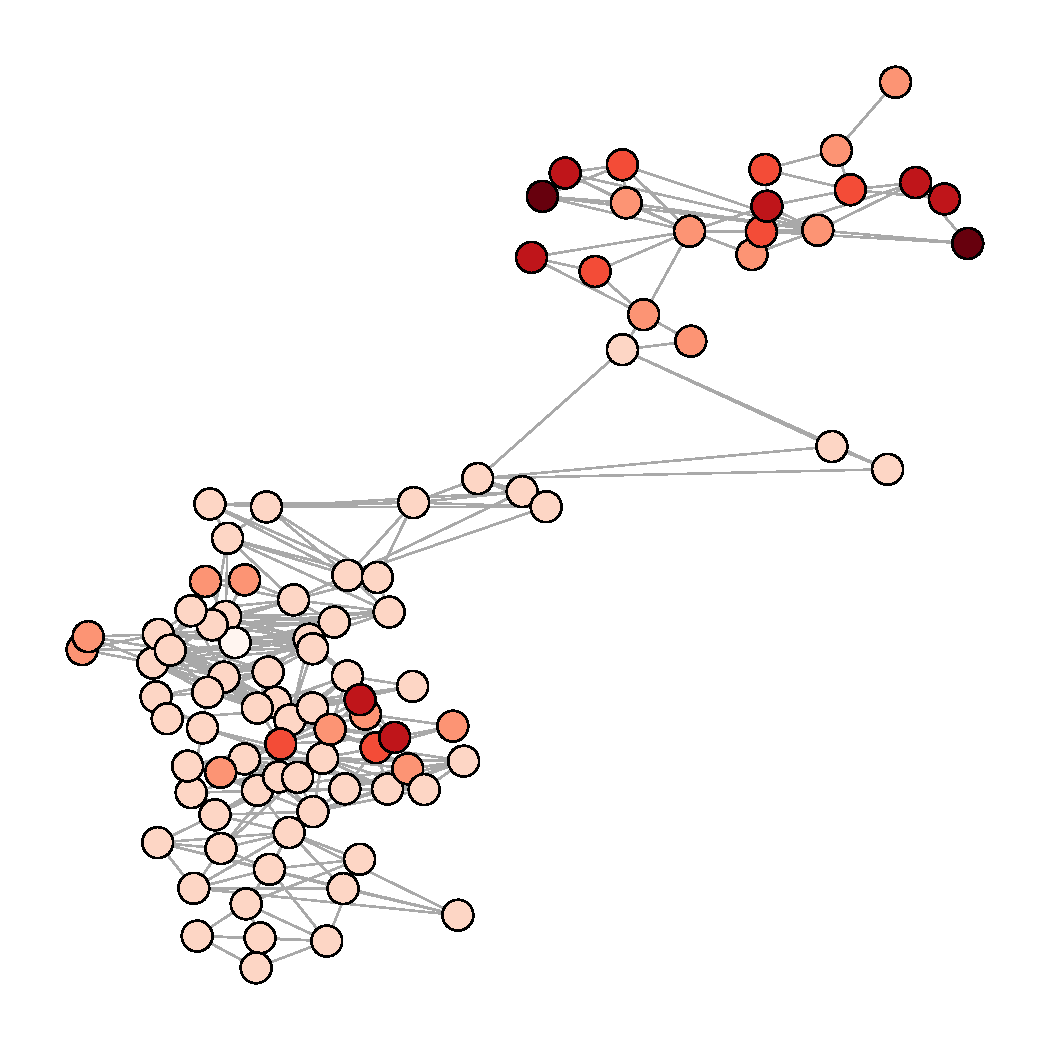
\includegraphics[width = 0.3\textwidth]{../Figure/brain1_z.pdf}
\caption{Subnetwork of MRI network. Darker colored nodes indicate higher positioned node in terms of $x$-axis(left), $y$-axis(middle), and $z$-axis(right).}
\end{figure}


%%%%%%%%%%%%%%%%%%%%%%%%%%%%%%%%%%%%%%%%%%%%%%%%%%%%%%%%%%%%%%%%
\newpage
\section{Discussions}
\label{sec:discussion}



\subsection{[dis1]}


Throughout this study, we demonstrate that multiscale network test statistic to test network independence performs well in diverse settings, being supported by thorough theory on distance correlation and diffusion maps. 
Testing independence is often the very first step in investigating relationship between network topology and nodal attributes in our interest. It is more likely that we want to know more than binary decision of rejecting or not rejecting the hypothesis. Multiscale test statistics due to both neighborhood choice $\{ (k,l)  \}$ and time spent in diffusion processes $\{ t \}$ provides us a hint on latent dependence structure as well.  


\subsection{[dis2]}

	Due to the ambiguousness of saying \textit{optimal}, our work has some limitations; we do not suggest any theoretically supported tools to select the \textit{optimal} time to obtain p-values of test statistics or maybe we want a family of p-values as a function of $t$. Further research can be focused on restoring true dependence pattern or estimating \textit{optimal} scale from a family of statistics. On the other hand, obtaining a full family of statistics are also computationally infeasible; at every Markov process, we chose the optimal region of neighborhood. As an ad hoc, we chose $t$ with highest power or lowest p-values from 1 to 10 for our simulation \ref{sec:sim}.  
	
	Other than these computational issues, someone might be uncomfortable about being conditioned by a random function of $g$ and $\eta$.  However, this is inevitable for arguing sample properties of being \textit{i.i.d.}, which is also very conceptual and impossible to prove. By conditioning diffusion maps $\{ \mathbf{U}_{t} \}$ by unknown network generative model $g(\cdot, \cdot)$ and also unknown diffusion process model $\eta(\cdot)$, we are finally able to assert that our observations are a fair sample eligible for test. 
	
	 

\subsection{[dis3]}

	Despite a few shortcomings listed above, a range of applications of \textit{MNT} statistics and multiscale representation of network is very diverse. Especially multiscale version of test would be very useful when indirect networking not directly from edge is not ignorable or cluster membership significantly affects attributes. 
	
	Furthermore even though we specifically constraint the statistic into testing independence between network and nodal attributes, we can now do independence testing of two networks with same size by inputting diffusion distance at each time point from each of network in equation \ref{eq:MGC}. This type of test would be useful when we want to show a pair of networks are topologically or structurally independent. For example, we might wonder if network on \textit{Facebook} and network induced by club activity within class or school are independent or not. 

	







%%%%%%%%%%%%%%%%%%%%%%%%%%%%%%%%%%%%%%%%%%%%%%%%%%%%%%%%%%%%%%%%
\newpage
\appendix
\section{appendix}

\subsection{[apd1]}
\begin{itemize}
	\item {\it  [apd1] additional plots   \/}
\end{itemize}


\begin{equation}
\begin{gathered}
X_{i} \overset{i.i.d}{\sim} Multi(1/3, 1/3, 1/3), i = 1,2, ... , n \\ 
Z_{i}  \sim  \left\{  \begin{array}{ccc} Multi(1/2, 1/4, 1/4) & X_{i} = 1 \\ Multi(1/4, 1/2, 1/4) & X_{i} = 2 \\ Multi(1/4, 1/4, 1/2) & X_{i} = 3  \end{array} \right. \\
A_{z_{i}, z_{j}} \sim Bern \left[  \begin{array}{ccc}   0.5 & 0.2 &  0.2  \\ 0.2 & 0.5 & 0. 2  \\ 0.2 & 0.2 & 0.2  \end{array}  \right]
\end{gathered}
\end{equation}




\subsection{[apd2]}
\begin{itemize}
	\item {\it  [apd2] (proof of) lemmas and theorems   \/}
\end{itemize}


\begin{theorem}[de Finetti's Theorem] 
\label{finetti}

1. Let $X_{1}, X_{2}, ...$ be an infinite sequence of random variables with values in a space $\mathbf{X}$. The sequence $X_{1}, X_{2}, ...$ is exchangeable if and only if there is a random probability measure $\eta$ on $\mathbf{X}$ such that the $X_{i}$ are conditionally i.i.d. given $\eta$. 

2. If the sequence is exchangeable, the empirical distributions

$$\hat{S}_{n} ( . ) := \frac{1}{n} \sum\limits_{i=1}^{n} \delta_{X_{i}} ( .), n \in \mathbb{N}$$
converges to $\eta$ as $n \rightarrow \infty$ with probability 1.
\end{theorem}

\begin{theorem}[Aldous Hoover Theorem]
	\label{Aldous_Hoover}

Let $\mathbf{A} = \{A_{ij}\}, 1 \leq i,j \leq \infty$ be a jointly exchangeable binary array if and only if there exists a random measurable function $f : [0,1]^{3} \rightarrow \mathbf{A}$ such that 

\begin{equation}
\big(  A_{ij}  \big) \stackrel{d}{=} \left( f \big( U_{i}, U_{j}, U_{ij} \big)  \right)
\end{equation}
where $(U_{i})_{i \in \mathbb{N}}$ and $(U_{ij})_{i,j > i \in mathbb{N}}$ with $U_{ij} = U_{ji}$ are a sequence and matrix, respectively, of i.i.d. Uniform[0,1] random variables. 
\end{theorem}



\begin{proof}[Proof of Lemma \ref{lemma1}]
By [Aldous-Hoover] Theorem\ref{Aldous_Hoover}, a random array $(A_{ij})$ is jointly exchangeable if and only if it can be represented as follows : 

There is a random function $g : [0,1]^2 \rightarrow [0,1]$ such that 

$$(A_{ij})  \stackrel{d}{=} Bern( g(W_{i}, W_{j}))$$
, where $W_{i} \overset{i.i.d.}{\sim} Uniform(0,1)$. Thus if $\mathbf{A}$ is an adjacency matrix of an undirected, exchangeable network, for any $i \leq j,$ $i,j = 1,... , n$:


\begin{equation}
\begin{split}
P \big(  A_{ij} = a_{ij} \big) & = \int P \big( A_{ij} \big| w_{i}, w_{j} \big) Pr(W_{i} = w_{i}) Pr(W_{j} = w_{j}) dw_{i} dw_{j} \\ & = \int_{0}^{1} \int_{0}^{1} g( w_{i},  w_{j})^{a_{ij}} \big( 1- g( w_{i},  w_{j}) \big)^{1-a_{ij}} dw_{i} dw_{j} 
\end{split}
\end{equation}

Then within each row, adjacent elements are independent and also identically distributed ,i.e. for fixed row index to $i \in \{1,2,... , n\}$,
$$P(A_{i1} = a_{i1}, A_{i2} = a_{i2}, ... , A_{in} = a_{in} ) = \prod\limits_{j=1}^{n} P(A_{ij} = a_{ij})$$

\end{proof}


\begin{proof}[Proof of Lemma \ref{lemma2}]
Based on Kallenberg and Exchangeable Graph (KEG) frameworks, introduced in \href{http://arxiv.org/abs/1512.03099}{[Veitch and Roy]}, a random array $(A_{ij})$ is jointly exchangeable if and only if it can be represented as follows : there is a random function $g : [0,1]^2 \rightarrow [0,1]$ such that 

\begin{equation}
(A_{ij})  \stackrel{d}{=} (A_{v_{i}, v_{j}} )  \stackrel{d}{=} Bern( g( \vartheta_{i}, \vartheta_{j}))
\end{equation}
, where $v_{i} \overset{i.i.d.}{\sim} Poisson(1), \vartheta_{i} \overset{i.i.d.}{\sim} Poisson(1), v_{i} \leq \nu, i = 1,2,... , n$, for some pre-specified $\nu >0$ so that finite size graphs can include vertices only if they participate in at least one edges. 

Thus if $\mathbf{A}$ is an adjacency matrix of an undirected, exchangeable network, for any $i \leq j,$ $i,j = 1,... , n$:


\begin{equation}
\begin{split}
P \big(  A_{ij} = a_{ij} \big) & = \int P \big( A_{ij} \big| v_{i}, v_{j} \big) Pr(V_{i} = v_{i}) Pr(V_{j} = v_{j}) Pr(\vartheta_{i} = \vartheta_{i}) Pr(\vartheta_{j} = \vartheta_{j})   dv_{i} dv_{j} d\vartheta_{i} d\vartheta_{j}   \\ & = \int_{0}^{\tau} \int_{0}^{\tau} \int_{0}^{\infty} \int_{0}^{\infty}  g( \vartheta_{i},  \vartheta{j})^{a_{ij}} \big( 1- g( \vartheta_{i},  \vartheta_{j}) \big)^{1-a_{ij}}  \\ & \quad \times dPois_{1}(x_{1}) \times dPois_{1}(x_{2}) \times dPois_{1}(x_{3}) \times dPoi_{1}(x_{4})  dx_{1} dx_{2} dx_{3} dx_{4}.
\end{split}
\end{equation}



\end{proof}


\begin{proof}[Proof of Lemma \ref{lemma3}]

We have shown that for fixed time $t$, diffusion distance is defined as an Euclidean distance of diffusion maps. Diffusion map is represented as follows :

\begin{equation}
\boldsymbol{U}_{t}(i) = \begin{pmatrix} \lambda^{t}_{1} \phi_{1}(i) & \lambda^{t}_{2} \phi_{2} (i)  & \cdots & \lambda^{t}_{q} \phi_{q}(i) \end{pmatrix} \in \mathbb{R}^{q}.
\end{equation}

,where $\Phi = \Pi^{-1/2}\Psi$ and $\mathbf{Q}=\mathbf{\Psi}\mathbf{\Lambda}\mathbf{\Psi}^{T} = \mathbf{\Pi}^{1/2} \mathbf{P} \mathbf{\Pi}^{-1/2}$. 
Thus $\mathbf{P \Pi^{-1/2} \Psi = \Pi^{-1/2} \Psi \Lambda}$. 

Then for any $r$th row ($r \in \{1,2, ... , q \}$, $(q \leq n)$), we can see that $P \phi_{r} = \lambda_{r} \phi_{r}$, where $\phi_{r} = \begin{pmatrix}  \frac{\psi_{r}(1)}{\sqrt{\pi(1)}} & \frac{\psi_{r}(2)}{\sqrt{\pi(2)}} & \cdots & \frac{\psi_{r}(n)}{\sqrt{\pi(n)}} \end{pmatrix}$.
Therefore to guarantee exchangeability (or i.i.d.) of $\mathbf{U}_{t}$, it suffices to show exchangeability (or i.i.d.) of $\mathbf{P}$.

Assume joint exchangeability of $\mathbf{G}$, i.e. $(A_{ij}) \stackrel{d}{=} \big( A_{\sigma(i) \sigma(j)} \big)$. 
Since $A_{ij}$ is binary, $\frac{A_{ij}}{\sum\limits_{ij} A_{ij}} = \frac{A_{ij}}{ 1 + \sum\limits_{l \neq j} A_{il}}$. Moreover, $A_{ij}$ and $(1 + \sum\limits_{l \neq j} A_{il})$ are independent given its link function $g$, and $A_{\sigma(i) \sigma(j)}$ and $(1 + \sum\limits_{l \neq j} A_{\sigma(i) \sigma(l)})$ are independent also given $g$.

Then the following joint exchangeability of transition probability holds:

\begin{equation}
\big( P_{ij} \big) = \left(  \frac{A_{ij}}{1 - A_{ij} + \sum\limits_{j=1}^{n} A_{ij} } \right)  \stackrel{d}{=} \left( \frac{A_{\sigma(i) \sigma(j)} }{1 - A_{\sigma(i) \sigma(j)} + \sum\limits_{\sigma(j) = 1}^{n} A_{\sigma(i) \sigma(j)} } \right) = \big( P_{\sigma(i) \sigma(j)} \big)
\end{equation}


Thus, transition probability is exchangeable. 
This results exchangeable eigenfunctions $\{ \Phi(1), \Phi(2), , ... , \Phi(n) \}$ 
where $\Phi(i) := \begin{pmatrix} \phi_{1}(i) & \phi_{2}(i) & \cdots & \phi_{q}(i) \end{pmatrix}^{T}$. Thus diffusion maps at fixed $t$, $\mathbf{U}_{t} = \begin{pmatrix} \Lambda^{t} \Phi(1)  & \Lambda^{t} \Phi(2) & \cdots & \Lambda^{t} \Phi(n)  \end{pmatrix}$ are exchangeable. 

Furthermore by de Finetti's Theorem(\ref{finetti}), we can say that $\mathbf{U}(t) = \{ U^{(t)}_{1}, U^{(t)}_{2}, ... , U^{(t)}_{n} \}$ are conditionally independent on a random probability measure $\eta$. 
\end{proof}


\begin{proof}[Proof of Theorem \ref{theorem1}]
\end{proof}


\begin{proof}[Proof of corollary \ref{corollary1}][Triangle inequality of diffusion distance]
\end{proof}

Let $x, y, z \in V(G).$

\begin{equation}
\begin{split}
 D^{2}_{t}(x,z) & = \sum\limits_{w \in V(G)} \big( P^{t}(x,w) - P^{t}(z,w)   \big)^2 \frac{1}{\pi(w)}  \\ & = \sum\limits_{w \in V(G)} \big(P^{t}(x, w) - P^{t}(y,w) + P^{t}(y,w) - P^{t}(z,w) \big)^2 \frac{1}{\pi(w)} \\ & = \sum\limits_{w \in V(G)} \big( P^{t}(x,w) - P^{t}(y,w) \big)^2 \frac{1}{\pi(w)}  + \sum\limits_{w \in V(G)} \big( P^{t}(y,w) - P^{t}(z,w)  \big)^2 \frac{1}{\pi(w)} \\ & + 2 \sum\limits_{w \in V(G)} \big( P^{t}(x,w) - P^{t}(y,w)  \big) \big( P^{t}(y,w) - P^{t}(z,w)  \big)\frac{1}{\pi(w)} \\ &= D^{2}_{t}(x,y) + D^{2}_{t}(y,z) +  2 \sum\limits_{w \in V(G)} \big( P^{t}(x,w) - P^{t}(y,w)  \big) \big( P^{t}(y,w) - P^{t}(z,w)  \big)\frac{1}{\pi(w)}   
\end{split}
\end{equation}


Thus it suffices to show that 

\begin{equation}
\sum\limits_{w \in V(G)} \big( P^{t}(x,w) - P^{t}(y,w)  \big) \big( P^{t}(y,w) - P^{t}(z,w)  \big)\frac{1}{\pi(w)} \leq D_{t}(x,y) \cdot D_{t}(y,z). 
\end{equation}

Let $a_{w} = \big(P^{t}(x,w) - P^{t}(y,w) \big) \sqrt{1 / \pi(w)}$ and $b_{w} = \big( P^{t}(y,w) - P^{t}(z,w) \big) \sqrt{1 / \pi(w)}$. Then the above inequality is equivalent to :

\begin{equation} 
\sum\limits_{w \in V(G)} a_{w} \cdot b_{w} \leq \sqrt{\sum\limits_{w \in V(G)} a^2_{w} \cdot \sum\limits_{w \in V(G)} b^2_{w} }.
\end{equation}

,which is true by Cauchy-Schwarz inequality.






%%%%%%%%%%%%%%%%%%%%%% Biobliography %%%%%%%%%%%%%%%%%%%%%%%%%%%%%%%%%
\newpage
\begin{thebibliography}{1}
	
	
	\bibitem{Orbanz} Orbanz, P., $\&$ Roy, D. M. (2015). Bayesian models of graphs, arrays and other exchangeable random structures. IEEE transactions on pattern analysis and machine intelligence, 37(2), 437-461.
	
	\bibitem{Caron}\hypertarget{Caron} Caron, F., $\&$ Fox, E. B. (2014). Sparse graphs using exchangeable random measures. arXiv preprint arXiv:1401.1137.
	
	\bibitem{Chan} Chan, S. H., Costa, T. B., $\&$ Airoldi, E. M. (2013, December). Estimation of exchangeable graph models by stochastic blockmodel approximation. In Global Conference on Signal and Information Processing (GlobalSIP), 2013 IEEE (pp. 293-296). IEEE.
	
	\bibitem{Hoff}\hypertarget{Hoff}{ Hoff, P. D., Raftery, A. E., $\&$ Handcock, M. S. (2002). Latent space approaches to social network analysis. Journal of the american Statistical association, 97(460), 1090-1098.}
	
	\bibitem{Kallenberg} Kallenberg, O. (1990). Exchangeable random measures in the plane. Journal of Theoretical Probability, 3(1), 81-136.
	
	\bibitem{Austin}\hypertarget{Austin}{ Austin, A., Linkletter, C., $\&$ Wu, Z. (2013). Covariate-defined latent space random effects model. Social Networks, 35(3), 338-346.}
	
	\bibitem{centrality1} Mantzaris, A. V., Bassett, D. S., Wymbs, N. F., Estrada, E., Porter, M. A., Mucha, P. J., ... $\&$ Higham, D. J. (2013). Dynamic network centrality summarizes learning in the human brain. Journal of Complex Networks, 1(1), 83-92.
	
	\bibitem{centrality2} Sporns, O., Honey, C. J., $\&$ Kötter, R. (2007). Identification and classification of hubs in brain networks. PloS one, 2(10), e1049.
	
	\bibitem{Lazarsfeld} Lazarsfeld, P. F, $\&$ Henry, N. W. (1968). Latent structure analysis. New York: Houghton, Mifflin.
	
	\bibitem{Coifman}\hypertarget{Coifman}  Coifman, R. R., $\&$ Lafon, S. (2006). Diffusion maps. Applied and computational harmonic analysis, 21(1), 5-30.
	
	\bibitem{HHG} Heller, R., Heller, Y., $\&$ Gorfine, M. (2012). A consistent multivariate test of association based on ranks of distances. Biometrika, ass070.

	
	\bibitem{Fosdick}\hypertarget{Fosdick} Fosdick, B. K., $\&$ Hoff, P. D. (2015). Testing and modeling dependencies between a network and nodal attributes. Journal of the American Statistical Association, 110(511), 1047-1056.
	
	\bibitem{Veitch} Veitch, V., $\&$ Roy, D. M. (2015). The class of random graphs arising from exchangeable random measures. arXiv preprint arXiv:1512.03099.
	
	\bibitem{Szekely2007} Székely, G. J., Rizzo, M. L., $\&$ Bakirov, N. K. (2007). Measuring and testing dependence by correlation of distances. The Annals of Statistics, 35(6), 2769-2794.
	
	
	\bibitem{Szekely2013} Székely, G. J., $\&$ Rizzo, M. L. (2013). The distance correlation t-test of independence in high dimension. Journal of Multivariate Analysis, 117, 193-213.
	
	
	\bibitem{Cencheng} Cencheng at al, Revealing the structure of dependency between multimodal datasets via multiscale generalized correlation.
	
	
	\bibitem{Lyons} Lyons, R. (2013). Distance covariance in metric spaces. The Annals of Probability, 41(5), 3284-3305.
	
	\bibitem{Lee} Lee, J. R. (2006). Distance scales, embeddings, and metrics of negative type. University of California, Berkeley.
	
	\bibitem{Tang} Tang, Minh, and Michael Trosset. "Graph metrics and dimension reduction." Indiana University, Indianapolis, IN (2010).
	
	\bibitem{Lafon} Lafon, S., $\&$ Lee, A. B. (2006). Diffusion maps and coarse-graining: A unified framework for dimensionality reduction, graph partitioning, and data set parameterization. IEEE transactions on pattern analysis and machine intelligence, 28(9), 1393-1403.
	
	\bibitem{Karrer} Karrer, B., $\&$ Newman, M. E. (2011). Stochastic blockmodels and community structure in networks. Physical Review E, 83(1), 016107.
	

	
	
\end{thebibliography}




\end{document}